%% ==============================================
%%               Use Cases
%% ==============================================
%% Author: Fabian Sorn
%% ==============================================

\chapter{Use Cases}
\label{ch:usecases}

This chapter will give an overview over different scenarios that we will use for
the evaluation of the Plotting Libraries. All of these originate from teams at
CERN, that are looking into PyQt as an option to implement different \gls{gui}
applications, which also contain plots in them.


%% ==============================================
%%               BE-CO-HT
%% ==============================================
\section{Distributed Oscilloscope for BE-CO-HT}
\label{sec:usecases:becoht}

The first project interested in visualizing data using python graph libraries is
the Distributed Oscilloscope developed in the \gls{ht} section, who are
responsible for the development, production and support for the custom
electronic modules used in the Control System. The goal of the Digital
Oscilloscope is to synchronously monitor analog signals in a distributed system.
To achieve this synchronization, the signals from various sources are
time-stamped and sent to the \gls{gui}, where they can be displayed using
graphs. The project is distributed into three architectural layers, which are
depicted in figure \ref{fig:doarchitecture}.

\begin{figure}[h]
    \centering
    
\includegraphics[width=8cm]{resources/img/DoArchitecture}
    \caption{Digital Oscilloscope Architecture}
    \label{fig:doarchitecture}
\end{figure}

The layer closest to the hardware the depicted signals originate from, are the
device applications, which provide access to hardware resources. The central
layer is the Digital Oscilloscope Server, which is responsible for managing all
connections between device and user applications. The last layer closest to the
users are the user applications. The application our use case originates from,
is a \gls{gui} application representing a oscilloscope, a device for displaying
varying signal voltages over time. A screenshot of this application can be seen
in figure \ref{fig:dogui}.
\cite{DistrOscDocs, BeCoHtSection}

\begin{figure}[h]
    \centering
    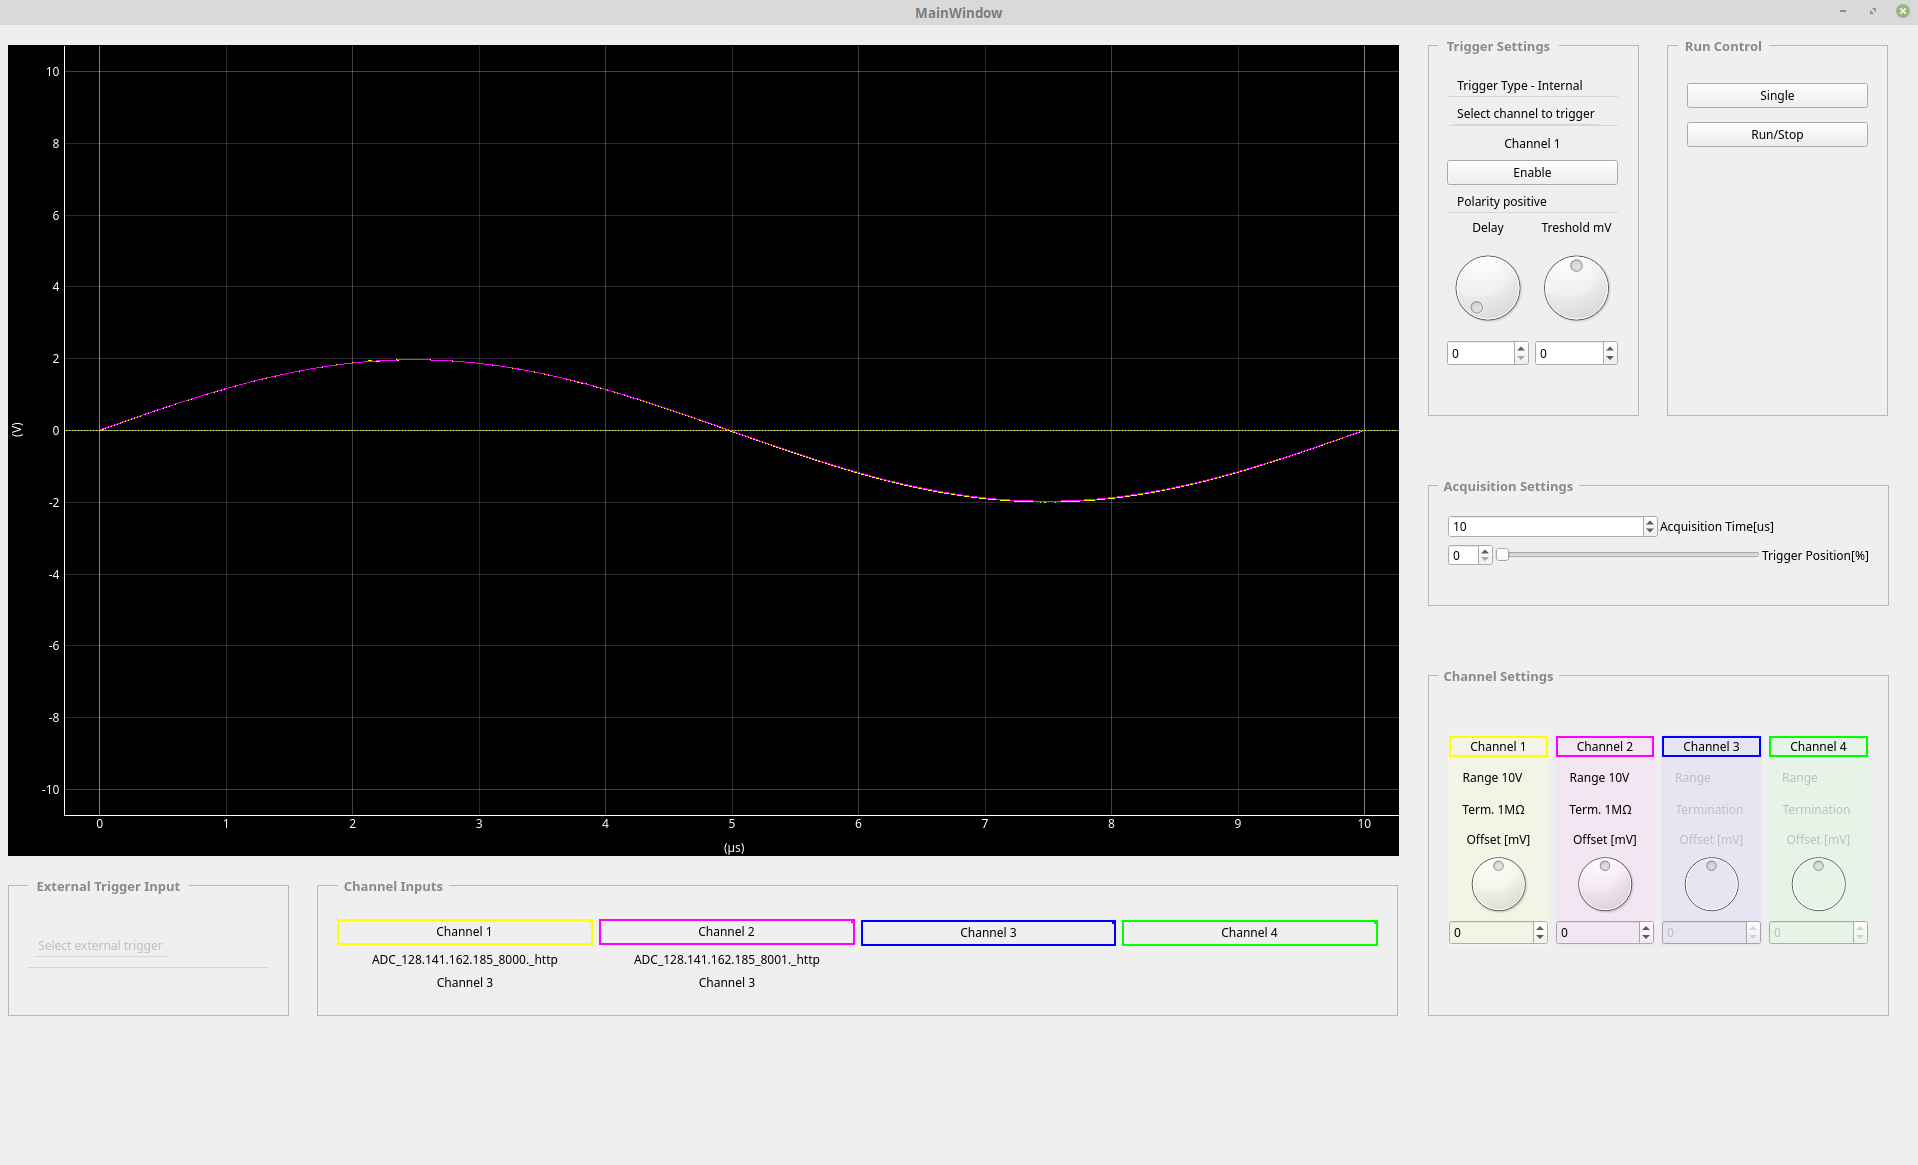
\includegraphics[width=15cm]{resources/img/DistributedOscilloscope}
    \caption{
        Distributed Oscilloscope GUI application displaying two analog signals
    }
    \label{fig:dogui}
\end{figure}

For this \gls{gui}, \gls{ht} is interested in displaying a plot in their
application, which is showing up to eight curves with up to 100.000 points per
curve. The goal for this graph would be an update rate of 25 updates per second.


%% ==============================================
%%               BE-OP-LHC
%% ==============================================
\section{Line Charts in section BE-OP-LHC}
\label{sec:usecases:becolhc}

The second Use Case we will investigate is coming from the \gls{lhcop}, who are
interested in displaying a Line Graph containing 3000 datasets displayed as
curves, who each will contain 2 * 3600 points. The data will be updated every
second.


%% ==============================================
%%               BE-CO-APS
%% ==============================================
\section{Use case in Linac4 Source GUI}
\label{sec:usecases:linac}

The third use case originates from \gls{aps}. For this, multiple scatter plots
should be displayed. The \gls{gui} Application will contain 4 different scatter
plots, each containing up to 3 data sets, which each contain 1 hour of live
data, which receives a new point roughly every 1.2 seconds. This results in 3000
visible points per data set.

\begin{figure}[h]
    \centering
    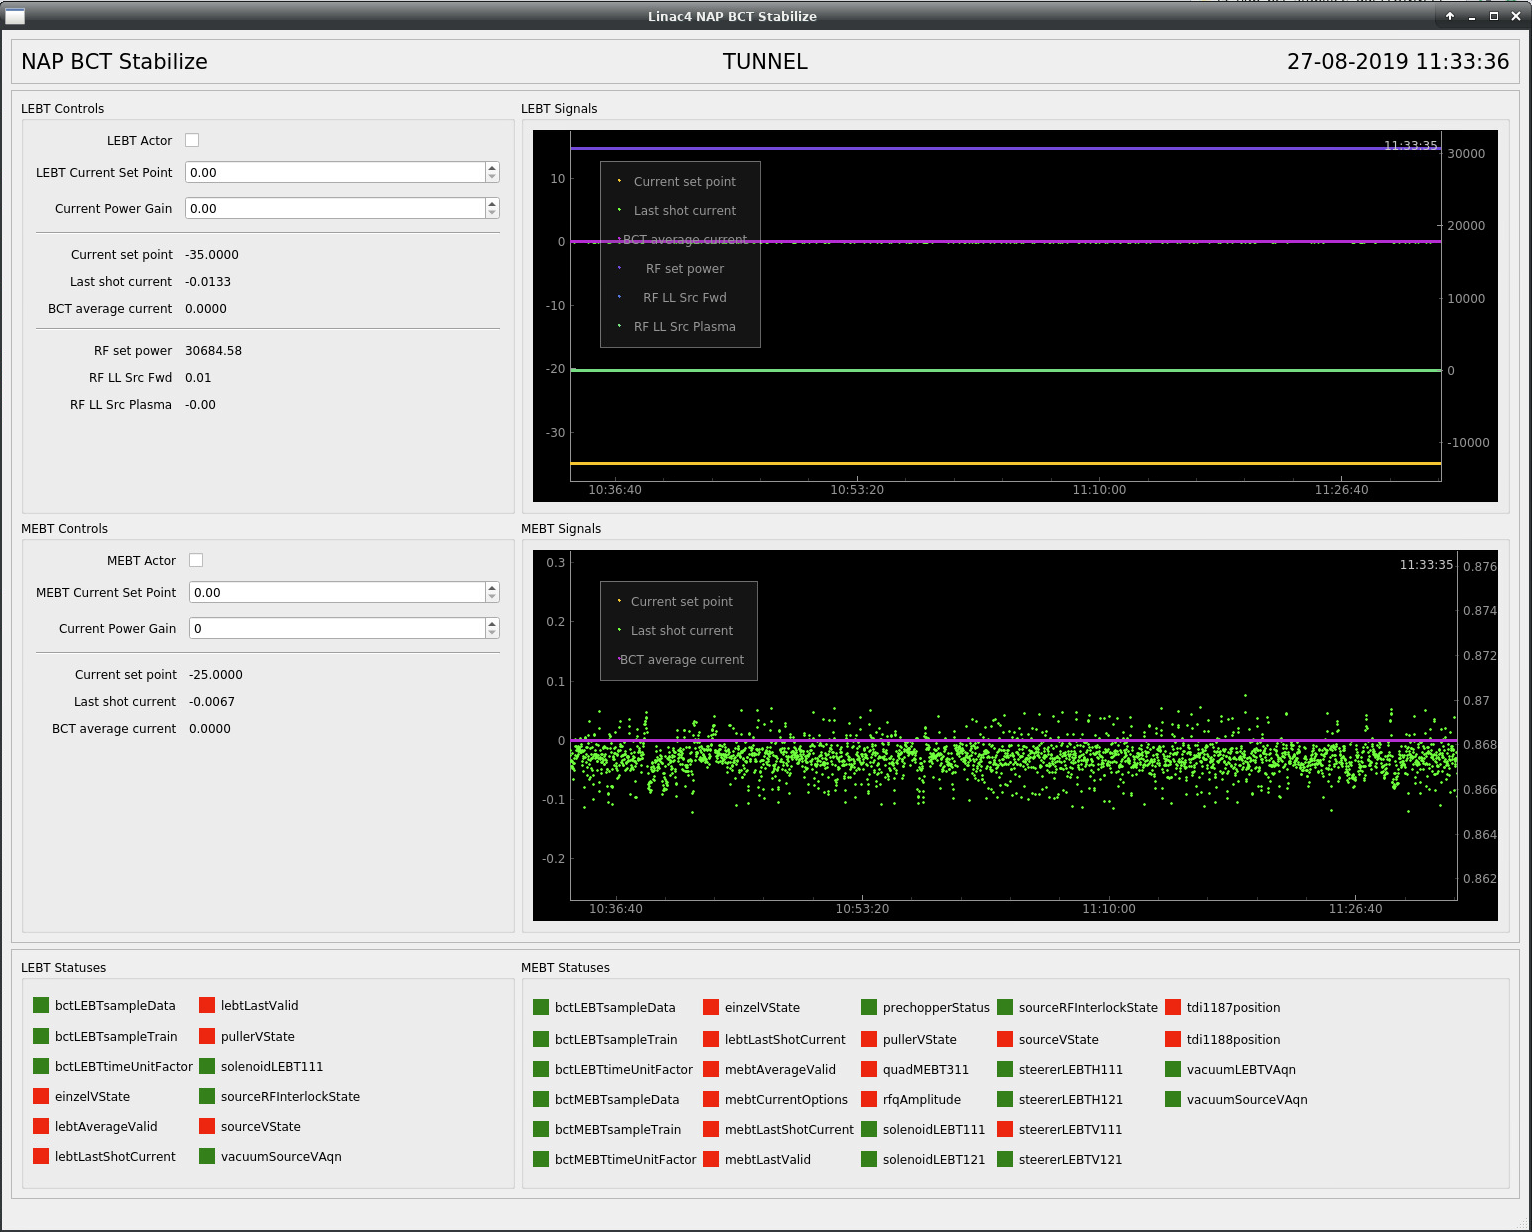
\includegraphics[width=15cm]{resources/img/Linac4SourceGui}
    \caption{Screenshot of the Linac4 Source Gui}
    \label{fig:linac4sourcegui}
\end{figure}

The Application where this Use Case is originated from is a \gls{gui} for the
Linear Accelerator Linac4, whose tasks it is to boost negative hydrogen ions to
high energies. The GUI will allow monitoring and manipulation of different
device settings. Image \ref{fig:linac4sourcegui} shows a screenshot of an early
version of the application with multiple scatter plots in the upper right part
of the window.
\cite{LinacFour,LinacFourGuiPres}

%% ==============================================
%%       Performance Metrics from Use Cases
%% ==============================================
\section{Conclusion}
\label{sec:usecases:metrics}

All of these Use Cases have in common, that they are displaying live data, which
will be delivered with a certain frequency. This means that the graph has only a
certain time to redraw until the next bunch of data arrives. Even for
applications containing graphs, which are not updated regularly, the time it
takes the graph to redraw is very important for the user interaction. Slow
redraw times will lead to stuttering user interfaces. As a result our highest
priority when investigating the performance of plotting libraries should be the
redraw speed of the graph.
